\documentclass{article}
\usepackage[utf8]{inputenc}
\usepackage{minted}
\usepackage{hyperref}
\usepackage{graphicx}

\setlength{\parindent}{0cm}

\title{Wireless Workshop Handbook}
\author{Jack Leightcap, Connor Northway}
\date{March 2021}

\hypersetup{
	colorlinks=true,
	urlcolor=blue,
}

\begin{document}

\maketitle

\section{PCB Design}
Install KiCad. The project files can be found \href{https://github.com/cnorthway/d1-sensor-shield}{here}.

\section{Soldering}
You can find the interactive Bill of Materials \href{http://www1.coe.neu.edu/~cnorthwa/ibom.html}{here}.

\subsection{Passives}
Resistors and the photoresistor do not have an orientation, just check you're putting the right values in the right places!

\subsection{LEDs}
The silk-screened line on the PCB for LED footprints is on \textbf{cathode} side (ground).
The easiest way to align them is to take them out of the tape aligned -- the holes on the tape are \emph{always} on the \textbf{cathode} side (Fig. \ref{fig:ledtape}).
\begin{figure}[H]
	\centering
	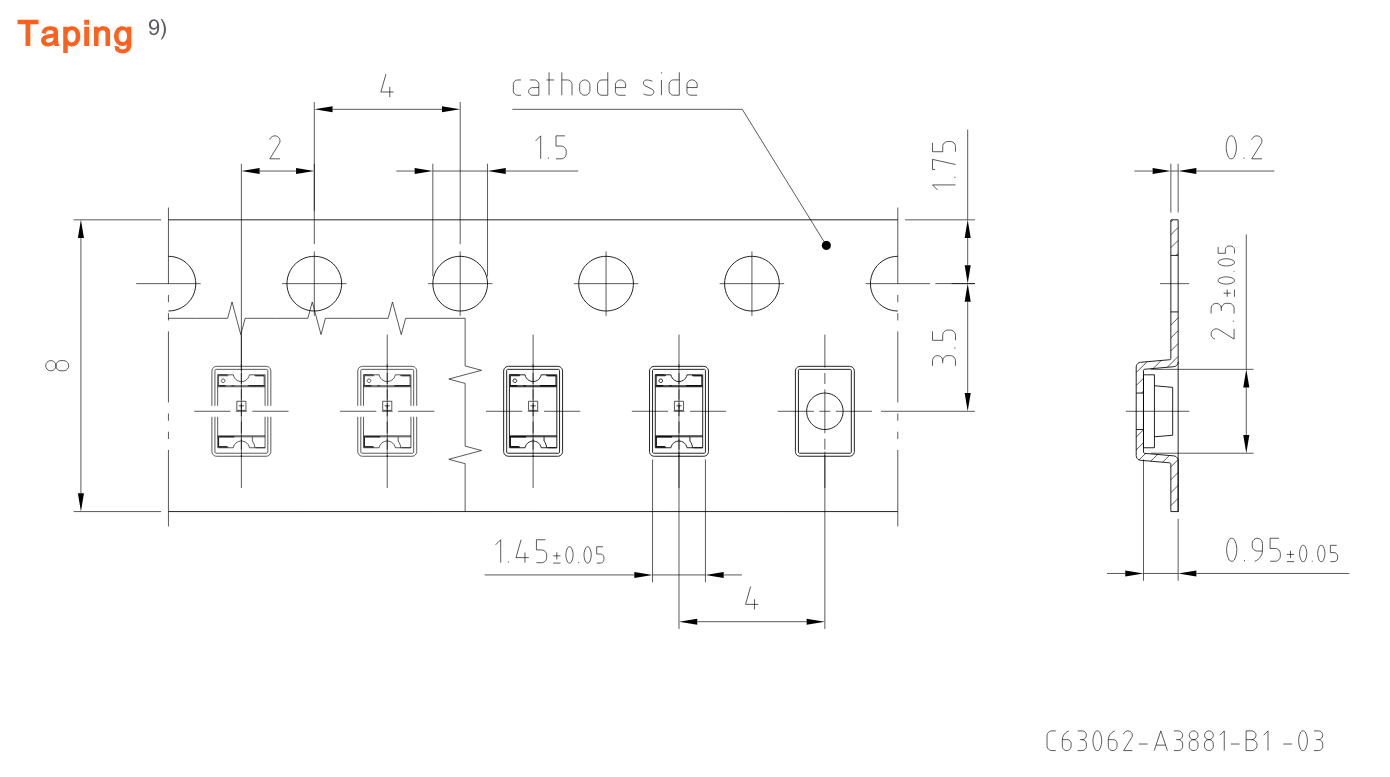
\includegraphics[width=12cm]{ledtape.png}
	\caption{LEDs oriented in tape}
	\label{fig:ledtape}
\end{figure}

\subsubsection{For when you inevitably drop one\ldots}
Both the green and orange LEDs have both a small dot in the metal and a green arrow that both point to their \textbf{cathode}.
The red LED is exactly the opposite, its markings point to its \textbf{anode}.
(Figs. \ref{fig:normal} and \ref{fig:red})

\begin{figure}[H]
	\centering
	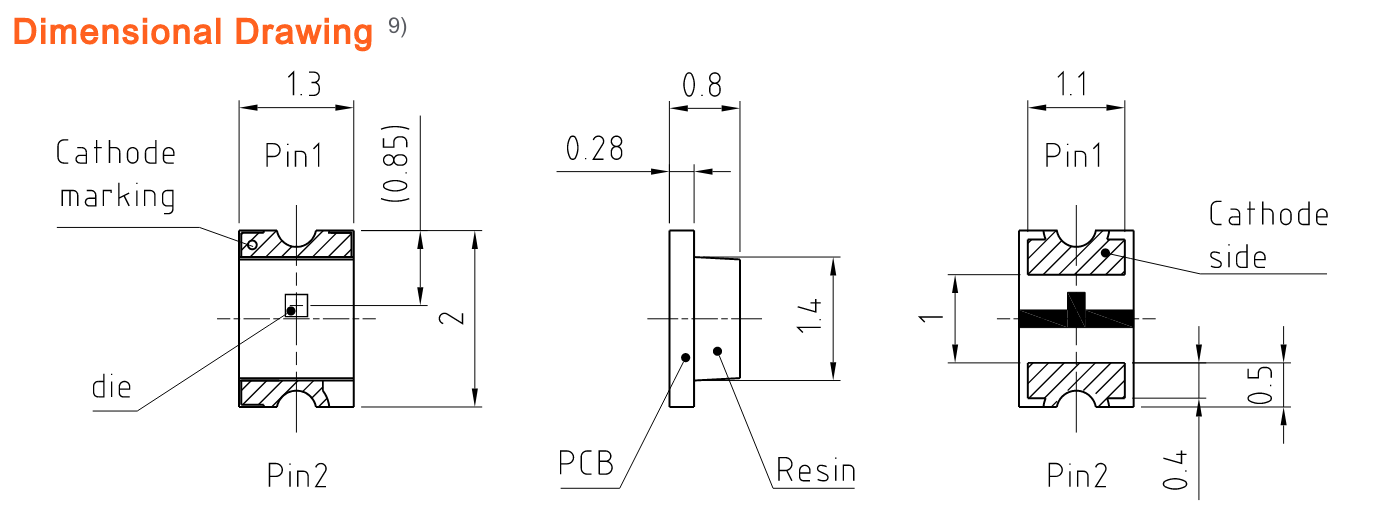
\includegraphics[width=12cm]{orange_green.png}
	\caption{Orange and green LEDs}
	\label{fig:normal}
\end{figure}
\begin{figure}[H]
	\centering
	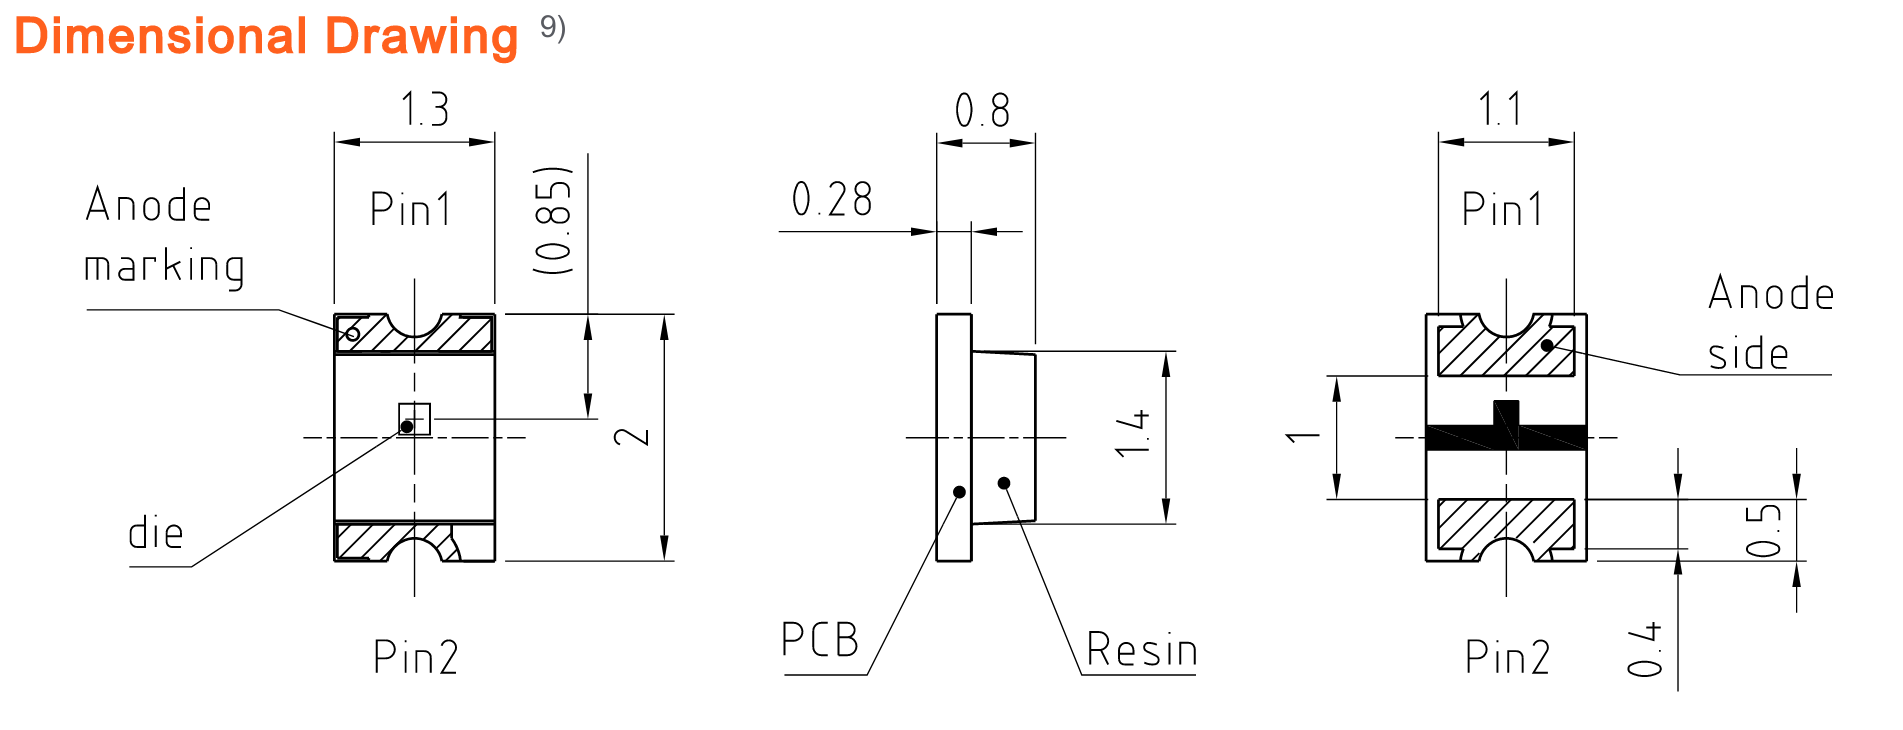
\includegraphics[width=12cm]{red.png}
	\caption{Red LEDs}
	\label{fig:red}
\end{figure}

\subsection{ICs}
Pin 1 for ICs are denoted with a longer silk-screened line on the PCB.
See figures \ref{fig:spi} and \ref{fig:temp} for the on-chip pin 1 markings.

\begin{figure}[H]
	\centering
	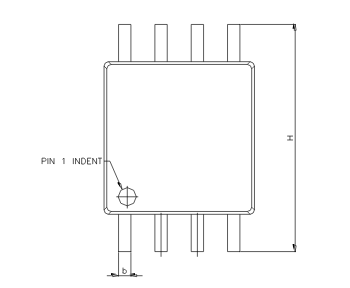
\includegraphics[width=5cm]{spi_pin1.png}
	\caption{Pin 1 mark on SPI Flash}
	\label{fig:spi}
\end{figure}
\begin{figure}[H]
	\centering
	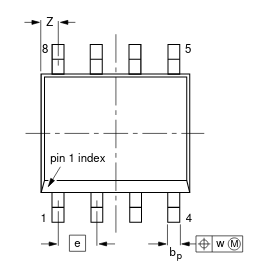
\includegraphics[width=4cm]{temp_pin1.png}
	\caption{Pin 1 mark on LM75B
		temperature sensor}
	\label{fig:temp}
\end{figure}
\subsection{Header Pins}
\begin{figure}[H]
	\centering
	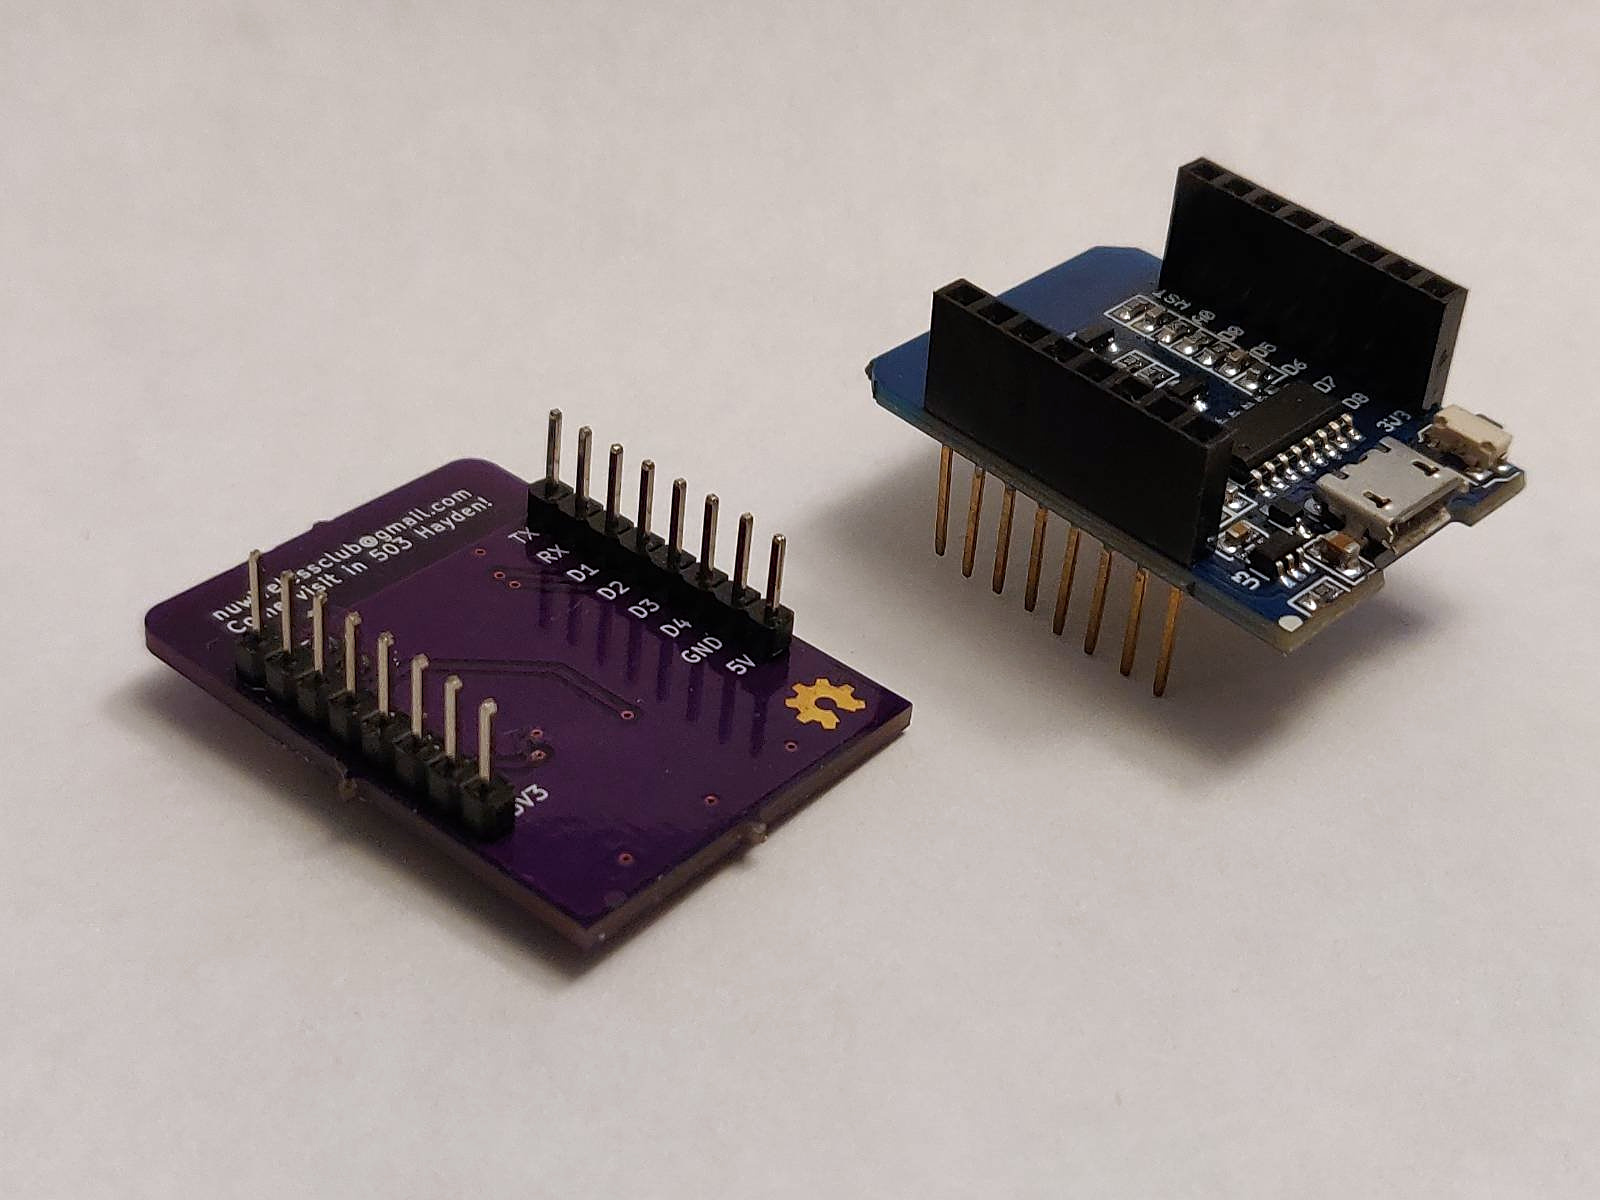
\includegraphics[width=12cm]{headers.jpg}
	\caption{Install
		the header
		pins as
		shown.}
	\label{fig:headerpin}
\end{figure}

\newpage

\section{Embedded Systems Programming}

First, get the firmware binary \href{http://www1.coe.neu.edu/~cnorthwa/workshop.bin}{here}.
To flash, use \texttt{\href{https://pypi.org/project/esptool/}{esptool}}:
assuming \texttt{pip} is using Python 3,

\begin{minted}
[ frame=lines, framesep=2mm, baselinestretch=1.2, fontsize=\footnotesize, ]
{bash}
 pip install esptool
# erase anything that's already on there
$ esptool.py erase_flash
# upload firmware $ esptool.py --baud 460800 write_flash \
 --flash_size=detect 0 workshop.bin
\end{minted}

There is in a shell script to automate the flash erasing/writing process \href{https://raw.githubusercontent.com/jleightcap/micropython/master/flash.sh}{here}.

Assuming the firmware was flashed successfully, pressing the reset button should blink the board LED five times.

To actually connect (not necessary to confirm flash is successful, assuming the LEDs flash) and get a Python REPL, using \texttt{picocom} for example,
\begin{minted}
[ frame=lines, framesep=2mm, baselinestretch=1.2, fontsize=\footnotesize, ]
{bash}
$ picocom /dev/ttyUSB0 -b115200
...
Type [C-a] [C-h] to see available commands
Terminal ready
>>> import os
>>> os.listdir()
['boot.py', 'inet.py', 'led.py', 'light.py', 'temp.py']
>>>
\end{minted}

\end{document}
